\documentclass[ignorenonframetext,]{beamer}
\setbeamertemplate{caption}[numbered]
\setbeamertemplate{caption label separator}{: }
\setbeamercolor{caption name}{fg=normal text.fg}
\beamertemplatenavigationsymbolsempty
\usepackage{lmodern}
\usepackage{amssymb,amsmath}
\usepackage{ifxetex,ifluatex}
\usepackage{fixltx2e} % provides \textsubscript
\ifnum 0\ifxetex 1\fi\ifluatex 1\fi=0 % if pdftex
  \usepackage[T1]{fontenc}
  \usepackage[utf8]{inputenc}
\else % if luatex or xelatex
  \ifxetex
    \usepackage{mathspec}
  \else
    \usepackage{fontspec}
  \fi
  \defaultfontfeatures{Ligatures=TeX,Scale=MatchLowercase}
\fi
% use upquote if available, for straight quotes in verbatim environments
\IfFileExists{upquote.sty}{\usepackage{upquote}}{}
% use microtype if available
\IfFileExists{microtype.sty}{%
\usepackage{microtype}
\UseMicrotypeSet[protrusion]{basicmath} % disable protrusion for tt fonts
}{}
\newif\ifbibliography
\hypersetup{
            pdftitle={Ajustes Automáticos},
            pdfauthor={Rafael La Buonora},
            pdfborder={0 0 0},
            breaklinks=true}
\urlstyle{same}  % don't use monospace font for urls
\usepackage{graphicx,grffile}
\makeatletter
\def\maxwidth{\ifdim\Gin@nat@width>\linewidth\linewidth\else\Gin@nat@width\fi}
\def\maxheight{\ifdim\Gin@nat@height>\textheight0.8\textheight\else\Gin@nat@height\fi}
\makeatother
% Scale images if necessary, so that they will not overflow the page
% margins by default, and it is still possible to overwrite the defaults
% using explicit options in \includegraphics[width, height, ...]{}
\setkeys{Gin}{width=\maxwidth,height=\maxheight,keepaspectratio}

% Prevent slide breaks in the middle of a paragraph:
\widowpenalties 1 10000
\raggedbottom

\AtBeginPart{
  \let\insertpartnumber\relax
  \let\partname\relax
  \frame{\partpage}
}
\AtBeginSection{
  \ifbibliography
  \else
    \let\insertsectionnumber\relax
    \let\sectionname\relax
    \frame{\sectionpage}
  \fi
}
\AtBeginSubsection{
  \let\insertsubsectionnumber\relax
  \let\subsectionname\relax
  \frame{\subsectionpage}
}

\setlength{\parindent}{0pt}
\setlength{\parskip}{6pt plus 2pt minus 1pt}
\setlength{\emergencystretch}{3em}  % prevent overfull lines
\providecommand{\tightlist}{%
  \setlength{\itemsep}{0pt}\setlength{\parskip}{0pt}}
\setcounter{secnumdepth}{0}

\title{Ajustes Automáticos}
\author{Rafael La Buonora}
\date{25/1/2021}

\begin{document}
\frame{\titlepage}

\begin{frame}{(Börsch-Supan 2007): Opciones de diseño en los sistemas
previsionales}

\begin{itemize}
\tightlist
\item
  Sostenibilidad Financiera
\item
  Efectos sobre la oferta laboral
\item
  Distribución del ingreso.
\end{itemize}

\end{frame}

\begin{frame}{(Börsch-Supan 2007): Aspectos más salientes}

\begin{itemize}
\tightlist
\item
  Reparto vs.~Ahorro
\item
  Contribución Definida vs.~Beneficio Definido.
\end{itemize}

Los sistemas previsionales deben encontrar el mix óptimo entre las
distintas propiedades de los sistemas.

\end{frame}

\begin{frame}{(Börsch-Supan 2007): Sistemas de Reparto y Beneficio
Definido}

\begin{itemize}
\tightlist
\item
  Ofrecen seguridad sobre los ingresos de los jubilados
\item
  Solidaridad intergeneracional
\item
  Vulnerables al riesgo demográfico (relación de dependencia)
\item
  En estos sistemas la variable de ajuste es la tasa de contribución.
\end{itemize}

\end{frame}

\begin{frame}{(Börsch-Supan 2007): Beneficio no tan definido}

\begin{itemize}
\tightlist
\item
  Las presiones demográficas vuelven los aumentos en las tasas de
  contribución demasiado altos.
\item
  Es necesario reducir los beneficio para mantener la sostenibilidad de
  los sistemas.
\item
  Hay una gama de sistemas intermedios entre Beneficio Definido y
  Contribución Definida, que permiten ajustar el equilibrio entre la
  seguridad de las prestaciones y la sostenibilidad del sistema.
\end{itemize}

\end{frame}

\begin{frame}{(Börsch-Supan 2007): La edad de retiro}

\begin{itemize}
\item
  La relación de dependencia puede alterarse via cambios en la edad de
  reitro.
\item
  Una idea natural es indexar la edad mínima de retiro a la esperanza de
  vida.
\item
  Hay un alto grado de incertidumbre sobre el aumento futuro en la
  esperanza de vida.
\item
  Esto hace que aumentar la edad de retiro mediante un esquema fijo
  (Alemania, EUA) no sea deseable
\item
  Un compromiso razonable puede ser mantener fija la proporción de la
  vida que las personas pasan retiradas.
\end{itemize}

\end{frame}

\begin{frame}{(Börsch-Supan 2007): Proyección de la tasa de dependencia}

\begin{figure}
\centering
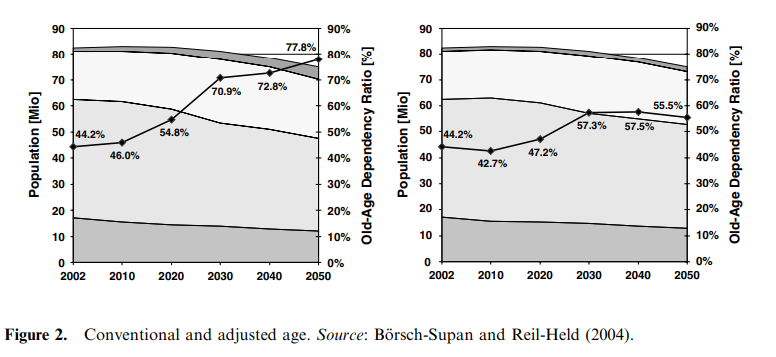
\includegraphics{imgs_reforma/borsch.png}
\caption{}
\end{figure}

\end{frame}

\begin{frame}{(Börsch-Supan 2007): Opciones}

Las reformas tienen solo 4 opciones para ajustarse al envejecimiento
demográfico:

\begin{itemize}
\tightlist
\item
  Bajar las tasas de reemplazo
\item
  Aumentar las tasas de contribución
\item
  Aumentar las edades de retiro
\item
  Aumentar los niveles de ahorro previo.
\end{itemize}

\end{frame}

\begin{frame}{Caso Suecia}

\end{frame}

\begin{frame}{Caso Alemania}

\end{frame}

\begin{frame}{(Turner 2009): Ajustes Automáticos para restaurar la
solvencia}

\begin{itemize}
\tightlist
\item
  Las reformas ad-hoc tienen problemas para resolver los problemas de
  sostenibilidad de los sistemas previsionales.
\item
  Por lo menos 12 países implementaron algún cambio automático para
  indexar las prestaciones a la esperanza de vida.
\end{itemize}

\end{frame}

\begin{frame}{(Turner 2009): Los mecanismos}

\begin{itemize}
\tightlist
\item
  Frecuencia del ajuste
\item
  Cambios frecuentes (indexación de prestaciones iniciales a la
  esperanza de vida)
\item
  Evento disparador
\item
  El ajuste tiene efecto si algún indicador de solvencia pasa cierto
  umbral.
\item
  Disparador ``duro'' o ``blando''
\item
  El gobierno puede tener mayor o menor grado de acción en las medidas
  implementadas para restaurar el equilibrio
\item
  Mecanismo de ajuste
\item
  Tasas de contribución, tasas de reemplazo o edades de retiro.
\end{itemize}

\end{frame}

\begin{frame}{(Turner 2009): Indexación de los beneficios a la esperanza
de vida}

\begin{itemize}
\tightlist
\item
  Algunos países indexan alguno de los parámetros de la SS a la
  esperanza de vida.
\item
  De esta manera, los trabajadores estan protegidos del ``riesgo'' de
  sobrevida respecto a su cohorte.
\item
  Portugal y Japón reducen los beneficios al momento del retiro 1\% si
  la esperanza de vida aumenta 1\%.
\item
  Otro mecanismo utilizado consiste en reducir el monto actualizado de
  la Riqueza Jubilatoria en la misma medida que el aumento en la
  esperanza de vida.
\item
  Otro mecanismo es el aumento de la edad mínima con el aumento de la
  esperanza de vida. Se puede calibrar para mantener la relación de
  dependencia o el ratio de años retirado respecto al retiro.
\end{itemize}

\end{frame}

\begin{frame}{(Turner 2009): Experiencias de países}

\begin{itemize}
\tightlist
\item
  Países con sistemas de reparto que indexan las jubilaciones a la
  esperanza de vida (Portugal y Finlandia).
\item
  Países con Sistemas Nocionales (Italia y Polonia)
\item
  Sistemas que indexan la edad mínima de retiro a la esperanza de vida
  (Reino Unido y Dinamarca).
\item
  Países con mecanismos de ajustes atados a la solvencia del sistema
  (Suecia, Alemania, Japón, Canadá).
\item
  Otros mecanismos (Francia).
\end{itemize}

\end{frame}

\begin{frame}{(Turner 2009): Ventajas y Desventajas}

\end{frame}

\begin{frame}{(Turner 2009): Aspectos distributivos}

\end{frame}

\begin{frame}{(OCDE 2011): Linking Pensions to Life Expectancy}

\begin{itemize}
\tightlist
\item
  Contexto: aumento de la longevidad y sistemas de reparto
\item
  Muchas de las reformas recientes en los sistemas previsionales hacen
  ajustes automáticos de los parámetros a la esperanza de vida.
\item
  Además de los beneficios económicos, los ajustes automáticos pueden
  ser atractivos si hacen más viables la reducción de los beneficios
  políticamente.
\end{itemize}

\end{frame}

\begin{frame}{(OCDE 2011): Distintas formas de vincular las jubilaciones
a la esperanza de vida}

\begin{figure}
\centering
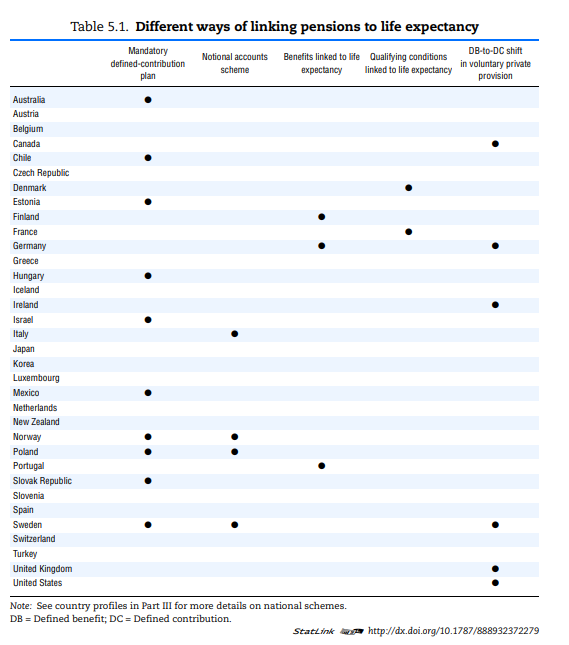
\includegraphics{imgs_reforma/ocde.png}
\caption{}
\end{figure}

\end{frame}

\begin{frame}{Sistemas de Contribución Definida}

\begin{itemize}
\tightlist
\item
  El capital pensionario acumulado se convierte en una anualidad.
\item
  La anualidad depende de la esperanza de vida del individuo.
\end{itemize}

\end{frame}

\begin{frame}{Sistemas Nocionales}

\begin{itemize}
\tightlist
\item
  También implican el cálculo de una anualidad.
\end{itemize}

\end{frame}

\begin{frame}{Monto de las jubilaciones vinculadas a la esperanza de
vida}

\begin{itemize}
\tightlist
\item
  Finlandia y Portgugal indexan el valor de las jubilaciones con un
  factor que depende de la esperanza de vida.
\item
  El sistema de puntos en Alemania ajusta el valor del punto a la
  relación demográfica del sistema.
\end{itemize}

\end{frame}

\begin{frame}{Condiciones de elegibilidad vinculadas a la esperanza de
vida}

\begin{itemize}
\tightlist
\item
  Dinamarca preveé vincular la edad mínima a la esperanza de vida a
  partir de 2027
\item
  Italia en 2015 y Grecia en 2020.
\end{itemize}

\end{frame}

\begin{frame}{Incertidumbre en las proyecciones de la esperanza de vida}

\begin{figure}
\centering
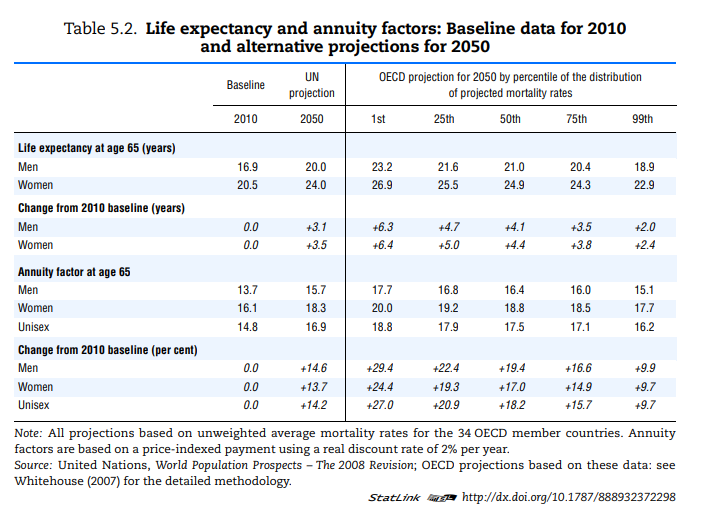
\includegraphics{imgs_reforma/esperanza.png}
\caption{}
\end{figure}

\end{frame}

\begin{frame}{Impacto de la mortalidad (1)}

\begin{figure}
\centering
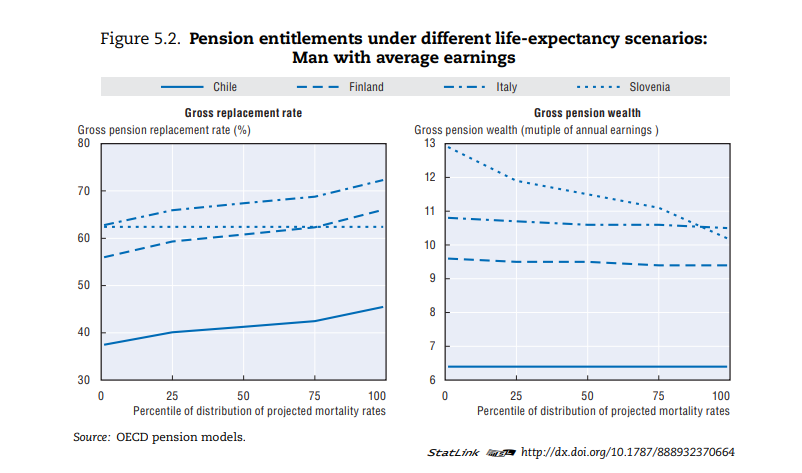
\includegraphics{imgs_reforma/morta.png}
\caption{}
\end{figure}

\end{frame}

\begin{frame}{(Guardiancich et al. 2019): Adopción de esquemas NDC}

\begin{figure}
\centering
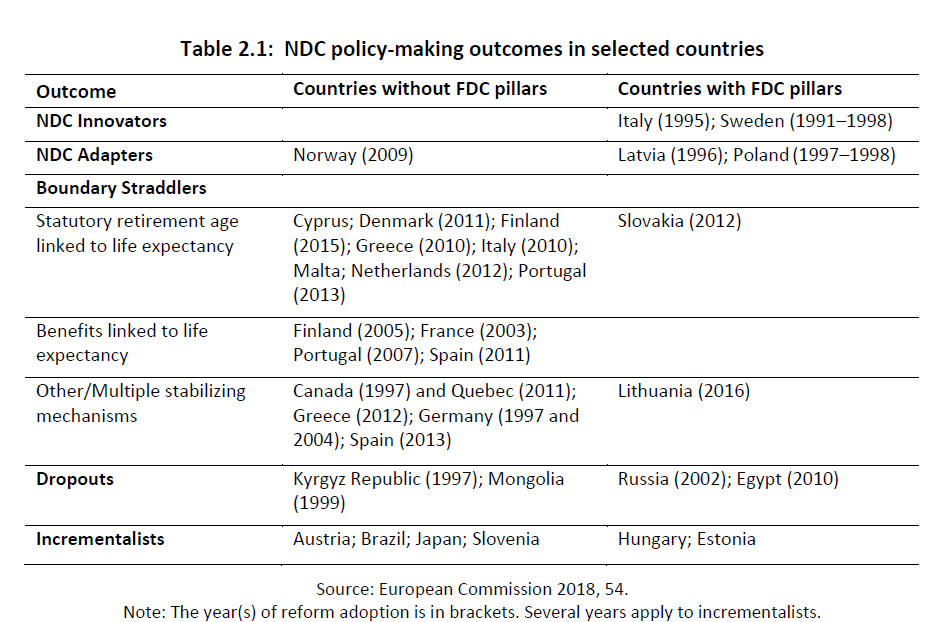
\includegraphics{imgs_reforma/reformas.png}
\caption{}
\end{figure}

\end{frame}

\end{document}
